\documentclass[10pt]{article}

\usepackage[T1]{fontenc}
\usepackage{lmodern}
\usepackage[utf8]{inputenc}
\input{glyphtounicode}
\pdfgentounicode=1
\usepackage{amsmath,amssymb,amsthm}
\usepackage{graphicx}
\usepackage[numbers,sort&compress]{natbib}
\usepackage[margin=1in]{geometry}
\usepackage{hyperref}
\usepackage{doi}

\hypersetup{
  colorlinks=true,
  linkcolor=blue,
  citecolor=blue,
  urlcolor=blue,
  pdftitle={When Warp Horizons Extend: Curvature Boundaries of Alcubierre Spacetimes},
  pdfauthor={Sergei Slobodov},
  pdfsubject={Parallel-propagated curvature singularities and the C2 extension alternative for stationary warp-drive spacetimes},
  pdfkeywords={warp drive, Alcubierre spacetime, curvature singularity, spacetime inextendibility, causal structure}
}

\newtheorem{theorem}{Theorem}
\newtheorem{proposition}[theorem]{Proposition}
\newtheorem{corollary}[theorem]{Corollary}
\theoremstyle{remark}
\newtheorem*{remark}{Remark}

\begin{document}

\title{When Warp Horizons Extend:\\
Curvature Boundaries of Alcubierre Spacetimes}

\author{Sergei Slobodov\\
  Independent researcher\\
  \href{mailto:sergei@slobodov.com}{\texttt{sergei@slobodov.com}}}

\date{\today}

\maketitle

\begin{abstract}
Conformal diagrams of a superluminal Alcubierre warp bubble appear to continue
beyond its front and rear horizons, but it is unclear whether that continuation
survives in the full four-dimensional geometry.  We compute the reduced diagram
explicitly for a smooth hyperbolic-secant profile and locate the finite-affine
endpoints of its horizon generators.  We then prove a general stationary result:
a null orbit of a complete Killing field with nonzero inaffinity and transverse
  tidal curvature ends at a parallel-propagated curvature singularity.  For
  nonpositive stationary scalar-shift warp drives, a global capture argument gives
  an exact alternative.  A proper Hausdorff \(C^2\) extension exists if and only if the
compact regular superluminal wall contains an open planar cap with constant
nonzero inaffinity.  Such a cap is a genuine Killing-horizon patch, and its
Kruskal continuation lifts through a finite transverse aperture.  Otherwise
the spacetime is \(C^2\)-inextendible.  The usual radial Alcubierre walls have no
such cap, so each corresponding four-dimensional spacetime is already its own
maximal Hausdorff \(C^2\) extension: the extra regions of the reduced diagram
have no regular four-dimensional counterpart.  The same local singular
mechanism occurs in a divergence-free Nat\'ario shift, showing that it is not
peculiar to scalar shifts.
\end{abstract}

\section{Introduction}

Alcubierre's metric realizes apparent superluminal motion of a compact
distortion at the cost of violations of the usual energy conditions
\cite{Alcubierre1994,PfenningFord1997,LoboVisser2004}.  Its null geodesics and
horizon structure have been studied extensively
\cite{ClarkHiscockLarson1999,BarceloEtAl2022}, as have quantum effects in
reduced models \cite{Hiscock1997,FinazziLiberatiBarcelo2009}.  The question here
is classical and global: does the continuation suggested by the reduced causal
diagram represent a continuation of the full four-dimensional spacetime?
Scalar polynomial invariants do not decide the issue, because they remain
finite at the relevant endpoints \cite{MattinglyEtAl2021,Rodal2023}.  A broader
classification of warp-drive geometries and their energy-condition properties
is given in Ref.~\cite{BarzegarBuchertVigneron2026}.

The paper has two main parts.  The first is an explicit conformal chart
for the reduced eternal geometry.  Earlier Kruskal-type and Misner-space
continuations \cite{GonzalezDiaz2000} and the standard diagram of Finazzi,
Liberati, and Barcel\'o \cite{FinazziLiberatiBarcelo2009} establish its causal
structure.  For the smooth hyperbolic-secant (sech) profile used here, both null
coordinates are elementary, so Section~\ref{sec:diagram} places the horizons,
representative worldlines, and finite-affine corners exactly.  This calculation
is independent of the class theorem and supplies its concrete Alcubierre
application.

The second part is a curvature-boundary and extension theorem.  The reduced geometry
genuinely continues through the finite-affine ends of its front and rear horizon
generators.  In four dimensions, however, a nonzero transverse tidal form at a
null orbit of a complete Killing field is amplified into a parallel-propagated
curvature singularity.  For scalar shifts, a Killing identity identifies this
form with the wall Hessian.  The Alcubierre endpoints therefore satisfy the
criterion even though all scalar curvature invariants remain finite.

A local singularity does not by itself exclude an extension attached elsewhere.
Section~\ref{sec:maximality} closes that gap for nonpositive stationary scalar shifts with a
compact regular superluminal wall.  Any regular extension would force an open
planar wall patch with constant inaffinity; conversely, such a patch has a
Kruskal extension.  This exact alternative implies that the reduced sech
diamond extends, whereas the original four-dimensional Alcubierre spacetime
does not.

\section{The Reduced Conformal Diagram}
\label{sec:diagram}

This section constructs the conformal diagram of the eternal geometry directly
from the metric.  For the smooth profile below every step is elementary, so the
diagram can be computed rather than sketched and the finite-affine corners can
be located explicitly.  To avoid conflict with the radial coordinate used
later, write \(\xi=x\) for the signed axial coordinate throughout this section.
We use the bubble-comoving convention: the usual lab-frame shift \(v_s f\)
becomes \(v=v_s(f-1)\) under \(x=X-v_st\), so the center has \(v=0\) and the
asymptotic exterior \(v=-v_s\).

Suppressing the transverse directions, the stationary comoving geometry reduces
to
\begin{equation}
  ds^2_{1+1}=-dt^2+[d\xi-v(\xi)dt]^2
    =-(1-v^2)dt^2-2v\,dt\,d\xi+d\xi^2 .
  \label{eq:reduced-metric}
\end{equation}
The two null families satisfy \(d\xi/dt=v\pm1\), so the retarded and advanced
null coordinates are
\begin{equation}
  u=t-\int\frac{d\xi}{v+1},\qquad
  w=t-\int\frac{d\xi}{v-1},
  \label{eq:null-coords}
\end{equation}
and inverting gives
\(dt=\tfrac12(1+v)du+\tfrac12(1-v)dw\),
\(d\xi=\tfrac12(1-v^2)(dw-du)\), hence the doubly null form
\begin{equation}
  ds^2_{1+1}=-(1-v^2)\,du\,dw .
  \label{eq:double-null}
\end{equation}
The horizons are the simple roots of \(1-v^2\).  For the even profile used
below, \(v\) decreases monotonically from \(0\) at the center to
\(-v_s<-1\) on each outward branch, so there are exactly two, at
\(\xi=\xi_1<0\) and \(\xi=\xi_2>0\) with \(v=-1\).  They divide the
reduced spacetime into the bubble interior, region II with \(|v|<1\), and the
two exterior branches, regions I and III with \(|v|>1\).

For the representative profile, written in the two-parameter form
\(v(\xi)=\alpha[\operatorname{sech}(\xi/a)-1\,]\) with \(\alpha>1\), both
integrals in Eq.~\eqref{eq:null-coords} are elementary.  With
\(\beta=\alpha/(\alpha-1)\), the horizons are
at \(\xi_{1,2}=\mp a\operatorname{arcosh}\beta\), the local peeling scale is
\(\kappa=(\alpha/a)\sqrt{\beta^2-1}/\beta^2\).  The closed-form
antiderivatives and regionwise compactifying map are recorded in
Appendix~\ref{app:sech-chart}; applying them gives
Figure~\ref{fig:reduced-patch}.

\begin{figure}[t]
  \centering
  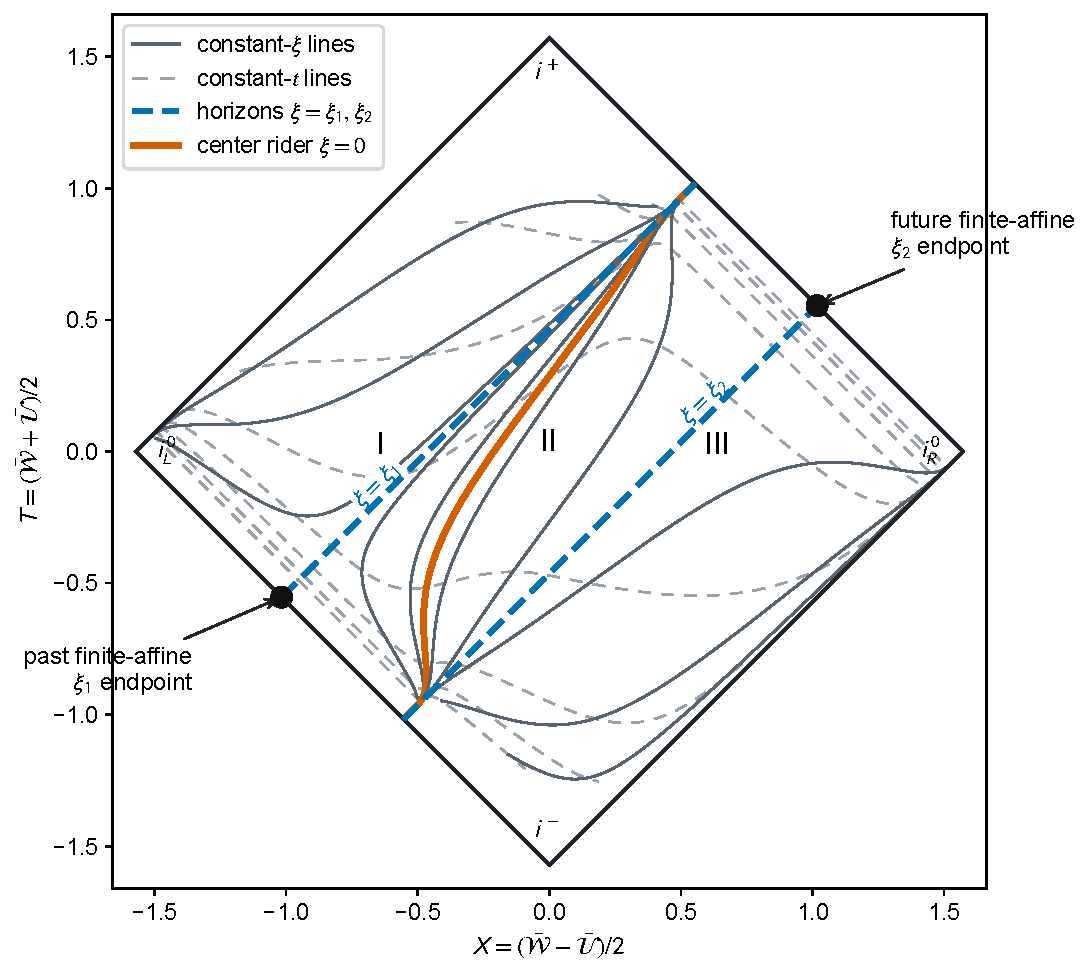
\includegraphics[width=0.82\linewidth]{figures/calculated_three_region_endpoint_patch.pdf}
  \caption{Calculated conformal diagram of the reduced \(1+1\) stationary
  patch for \(v(\xi)=2[\operatorname{sech}\xi-1]\).  The dark outer diamond is
  the compactification boundary.  The two thick short-dashed segments are the
  exact null horizons \(\xi=\xi_1,\xi_2\); they separate the bubble interior
  II, where \(|v|<1\), from the exterior branches I and III, where \(|v|>1\).
  Thin solid curves have constant \(\xi\) and are timelike in II and spacelike
  outside.  Light long-dashed curves are spacelike constant-\(t\) slices, and
  the thick solid central curve is the \(\xi=0\) rider.  The black dots mark
  the finite-affine past end of the \(\xi_1\) generator and future end of the
  \(\xi_2\) generator; their opposite ends have infinite affine parameter.
  The reduced metric extends through the marked corners, whereas transverse
  parallel-propagated curvature obstructs the corresponding continuation for
  a spatially finite \(3+1\) bubble.}
  \label{fig:reduced-patch}
\end{figure}

The corners are what the rest of the paper is about, so it is worth being
explicit about where they are and why they are reached at finite affine
parameter.  In the compactification of Appendix~\ref{app:sech-chart}, the
future \(\xi_2\) and past \(\xi_1\) generators terminate at the two marked
corners of Figure~\ref{fig:reduced-patch}.  Near \(\xi_2\), with
\(s=\xi-\xi_2\) and \(v=-1-\kappa s+O(s^2)\), one has
\(1-v^2=-2\kappa s+O(s^2)\) and
\(u=t+\kappa^{-1}\ln|s|+O(1)\), \(w=t+O(1)\).  The local chart
\begin{equation}
  U=
  \begin{cases}
    e^{\kappa u} & \text{region II},\\
    -e^{\kappa u} & \text{region III},
  \end{cases}
  \qquad V=e^{-\kappa w}
  \label{eq:endpoint-chart}
\end{equation}
then gives \(ds^2_{1+1}=[(1-v^2)/(\kappa^2UV)]\,dU\,dV\), whose prefactor has a
finite nonzero limit because \(UV\propto-s\).  The front generator is \(U=0\)
and its future endpoint is \(U=V=0\), at finite affine parameter; the
past-rear corner is analogous.  In the reduced geometry
\eqref{eq:double-null} the chart
\eqref{eq:endpoint-chart} is manifestly regular there, and the continuation
through the corner is the usual one.  Whether it survives restoring the
transverse directions is the subject of the rest of this paper.

\section{Curvature Boundaries and the Global \texorpdfstring{\(C^2\)}{C2} Extension Alternative}
\label{sec:maximality}

The reduced diagram raises two distinct extension questions.  Its front and
rear null generators end at finite affine parameter; a parallel-propagated
curvature singularity there excludes continuation through those particular
corners.  Global \(C^2\)-inextendibility is stronger, because a proper extension
might still attach elsewhere.  The theorem below identifies the two
possibilities for stationary scalar shifts.  Its global ingredients are a
controlled superluminal exterior and a compact regular stationary-limit wall.
The exceptional local geometry is an open piece of that wall which is itself a
constant-inaffinity Killing horizon.

\begin{theorem}[Scalar-shift extension alternative]
\label{thm:extension-alternative}
Let \(M=\mathbb R^4\) carry the scalar-shift metric
\begin{equation}
  ds^2=-dt^2+[dx-v(\boldsymbol{x})dt]^2+dy^2+dz^2,
  \qquad \boldsymbol{x}=(x,y,z),\quad r=|\boldsymbol{x}|,
  \label{eq:general-scalar-shift}
\end{equation}
where \(v\) is smooth, bounded, and \(v\leq0\).  Assume that, for some
\(v_s>1\), the exterior is either exactly constant or exponentially
short-range:
\begin{equation}
  v=-v_s\quad(r\geq R_0),
  \qquad\text{or}\qquad
  |v+v_s|+|\nabla v|\leq Ce^{-\sigma r}
  \quad(r\geq R_0),
  \label{eq:general-scalar-tail}
\end{equation}
for some \(R_0,C,\sigma>0\).  Suppose also that
\begin{equation}
  \Sigma=\{\boldsymbol{x}:v(\boldsymbol{x})=-1\}
  \label{eq:general-wall}
\end{equation}
is compact and regular.  Its stationary-generator locus is
\begin{equation}
  \mathcal G=\{p\in\Sigma:v_y(p)=v_z(p)=0\}
  \label{eq:generator-locus}
\end{equation}
The sign condition makes \(\Sigma=\{|v|=1\}\) the entire stationary-limit
set; it is not a coordinate normalization for profiles taking both signs.
Regularity implies \(v_x\ne0\) on \(\mathcal G\), so the theorem concerns
nondegenerate stationary generators.
Then \((M,g)\) admits a proper Hausdorff \(C^2\) Lorentzian extension if and
only if there are \(x_H\in\mathbb R\), a nonempty open disk
\(D\subset\mathbb R^2_{y,z}\), and a constant \(\kappa\ne0\) such that
\begin{equation}
  v(x_H,y,z)=-1,
  \qquad v_x(x_H,y,z)=-\kappa
  \quad ((y,z)\in D).
  \label{eq:planar-cap-criterion}
\end{equation}
When \eqref{eq:planar-cap-criterion} holds, the extension can be chosen smooth
and continues the finite-affine stationary generators through a bifurcate
Killing horizon over \(D\).  If no such disk exists, \((M,g)\) admits no proper
Hausdorff \(C^2\) Lorentzian extension.
\end{theorem}

The exterior and compactness assumptions capture any hypothetical extension
boundary.  The necessity of \eqref{eq:planar-cap-criterion} is a rigidity
statement: the uniform neighborhood of a regular endpoint forces the wall to
be planar and its inaffinity to be constant.  Its sufficiency is the ordinary
Kruskal construction, applied over a transverse disk.

\paragraph{Local finite-affine obstruction.}
For any Killing field \(\chi\), the Killing equation and Ricci identity give
\begin{equation}
  R(\chi,X,\chi,Y)
   =g(\nabla_X\chi,\nabla_Y\chi)
    -\frac12(\nabla^2\chi^2)(X,Y).
  \label{eq:killing-tidal-identity}
\end{equation}
For the scalar shift, take \(\chi=\partial_t\) and introduce the stationary
orthonormal frame
\begin{equation}
  e_0=\partial_t+v\partial_x,\qquad e_1=\partial_x,
  \qquad e_A=\partial_A.
  \label{eq:stationary-frame}
\end{equation}
On \(v=-1\),
\begin{equation}
  \nabla_{\partial_t}\partial_t
    =v_x\partial_t+v_y\partial_y+v_z\partial_z .
  \label{eq:not-whole-sphere}
\end{equation}
Thus \(\mathcal G\) is precisely the locus of null pregeodesic stationary
orbits, and \(e_0+e_1=\chi\) there.  At \(p\in\mathcal G\), the Killing
identity reduces to
\begin{equation}
  H_{AB}(p):=v_{AB}(p),
  \qquad
  R_{tAtB}=H_{AB},
  \qquad R_{KAKB}=H_{AB}q^2
  \quad\text{for }K=q\partial_t .
  \label{eq:screen-general}
\end{equation}

Let the null orbit through \(p\) be parametrized by Killing time and suppose
\(\nabla_\chi\chi=\alpha\chi\), with \(\alpha\ne0\).  At one end of the orbit,
its affine tangent \(K=q\chi\) obeys
\(|q|=[|\alpha|\,|\lambda-\lambda_*|]^{-1}\).  Thus a nonzero transverse tidal
form produces a parallel-propagated curvature singularity proportional to
\(|\lambda-\lambda_*|^{-2}\) at a finite-affine endpoint.  Such an endpoint
cannot be added in a \(C^2\) extension.  Applied to the front and rear generators
of Section~\ref{sec:diagram}, this shows that the marked corners of
Figure~\ref{fig:reduced-patch} are genuine four-dimensional curvature
boundaries, although the reduced metric continues through them.

\paragraph{Proof sketch: from capture to the extension alternative.}
If a proper extension existed, global hyperbolicity and
Ref.~\cite[Theorem~2]{GallowayLingSbierski2018} would supply a timelike geodesic
leaving \(M\) in finite proper time.  The capture proposition sends a boosted
subsequence toward \(p\in\mathcal G\).  Uniform curvature bounds on a small
transverse disk in the extension then force
\(v_{AB}-v_Av_B=0\) and \(v_{xA}=0\).  Thus \(e^{-v}\) is affine on the disk;
its gradient vanishes at \(p\), so \(v=-1\) and \(\kappa=-v_x\) is constant
there.  This is exactly Eq.~\eqref{eq:planar-cap-criterion}.

Conversely, that criterion makes the disk a constant-inaffinity Killing
horizon.  The explicit Kruskal coordinates in Appendix~\ref{app:global-proof}
extend it and give a proper Hausdorff attachment.  The appendix supplies the
capture, transverse-propagation, gluing, and past-end details.

\paragraph{A practical geometric test.}
The extendible alternative is exceptional: it requires the height function
\(x|_\Sigma\) to be constant on an open subset, and also requires constant
\(\kappa\) there.  Thus a Morse height function rules it out immediately.  The
older pointwise condition \(H_{AB}\ne0\) at every point of \(\mathcal G\) is a
convenient sufficient test, but is not the exact boundary between the two
cases.

\begin{corollary}[Radial Alcubierre maximality]
\label{cor:alcubierre-maximality}
Suppose \(v=v(r)\) is smooth and radially nonincreasing, with
\[
  v(0)=0,\qquad -v_s\leq v\leq0,\qquad
  v=-1\Longleftrightarrow r=R_F,
\]
and satisfies \eqref{eq:general-scalar-tail}.  Then the corresponding spacetime
is \(C^2\)-inextendible.  No nondegeneracy is assumed at \(R_F\).
\end{corollary}

\begin{proof}
Suppose that a proper extension exists.  Proposition~\ref{prop:capture} and the
transverse-rigidity argument through Eq.~\eqref{eq:forced-planar-wall} use
compactness of \(\Sigma\), but not its regularity.  They force an open planar
disk in \(\{v=-1\}\).  Here that level set is the sphere \(r=R_F\), which
contains no such disk, a contradiction.  For \(\kappa:=-v_r(R_F)\geq0\), the
wall Hessian at either pole is
\begin{equation}
  H_{AB}=-\frac{\kappa}{R_F}\delta_{AB}
  \label{eq:radial-hessian}
\end{equation}
and records the local tidal obstruction when \(\kappa>0\).
\end{proof}

This includes the sech family used in Section~\ref{sec:diagram} and the usual
smooth compact-transition profiles.  Each four-dimensional spacetime is
already its own maximal Hausdorff \(C^2\) extension: the larger continuation of
the stand-alone \(1+1\) metric does not lift to four dimensions.  No special
identity of the sech profile enters the proof, and no claim is made below
\(C^2\) regularity.


\section{Alcubierre, Wall Geometry, and a Nat\'ario Shift}

The preceding curvature analysis has three immediate applications: an exact
divergence for radial Alcubierre profiles, a geometric and source interpretation
of its coefficient, and a test of the local mechanism on a divergence-free
vector shift.

\paragraph{The Alcubierre endpoint.}
For a nondegenerate radial wall in Corollary~\ref{cor:alcubierre-maximality},
put \(\kappa=-v_r(R_F)>0\).  The
stationary field is null on \(v^2=1\), but the
four-dimensional wall is generally not null: there
\begin{equation}
  g^{ab}\partial_a(v^2-1)\partial_b(v^2-1)=4(v_y^2+v_z^2).
  \label{eq:wall-normal-norm}
\end{equation}
Equation~\eqref{eq:not-whole-sphere} therefore selects only the two axial
orbits.  At the future front, \(v_x=-\kappa\), so
\begin{equation}
  \nabla_{\partial_t}\partial_t=-\kappa\partial_t .
  \label{eq:nonaffine}
\end{equation}
The transverse vectors \(Y=\partial_y\) and \(Z=\partial_z\) are parallel
along this orbit.  Equations~\eqref{eq:radial-hessian} and
\eqref{eq:screen-general}, with
\(q=[\kappa(\lambda_*-\lambda)]^{-1}\), give
\begin{equation}
  R(K,Y,K,Y)=R(K,Z,K,Z)
  =-\frac{1}{\kappa R_F(\lambda_*-\lambda)^2}.
  \label{eq:main-blowup}
\end{equation}
The isometry \((t,x,y,z)\mapsto(-t,-x,y,z)\) gives the corresponding
past-rear result.  These are
parallel-propagated curvature singularities in the standard sense
\cite{EllisSchmidt1977}, although the stationary coordinate curvature and
scalar invariants remain finite.  Finite affine length alone is insufficient:
the analogous screen tensor vanishes in Painlev\'e--Gullstrand Schwarzschild,
whose Kruskal extension is regular \cite{LemosSilva2021}.

\paragraph{Wall geometry and source.}
Write a regular front locally as \(x=F(y,z)\).  Differentiating its wall
equation twice at a stationary generator gives
\begin{equation}
  F_{AB}=\frac{H_{AB}}{\kappa}.
  \label{eq:wall-graph-hessian}
\end{equation}
Thus \(H/\kappa\) is the graph Hessian.  In principal transverse coordinates
for a smooth convex front,
\begin{equation}
  F_{yy}=-C_1,\qquad F_{zz}=-C_2,\qquad C_i>0,
\end{equation}
and the spherical result is \(C_1=C_2=1/R_F\).  Vanishing of \(H\) at one
point only makes the wall flat to second order and does not ensure an
extension.  Theorem~\ref{thm:extension-alternative} requires the stronger, exact
geometry of an open planar cap with constant \(\kappa\).  On such a cap the
wall worldvolume is a genuine Killing horizon and the reduced continuation
lifts over its transverse disk.

The exceptional branch is compatible with a smooth compact wall; it is not an
artifact of the noncompact product \(v=v(x)\).  Appendix~\ref{app:compact-cap}
constructs a compact connected wall with exact planar caps and a constant
exterior.  Each cap admits a proper smooth Kruskal-product extension, while its
rim has no regular \(C^2\) endpoint.  Thus the exception is real but requires
exact geometry on an open set.

If the Einstein equation is imposed, the same wall tensor also controls the
affine null source projection (in geometrized units):
\begin{equation}
  8\pi T_{KK}=G_{KK}=q^2\operatorname{tr}H,
  \qquad
  G_{KK}=-\kappa(C_1+C_2)q^2<0
  \quad\text{at a convex future front}.
  \label{eq:null-source}
\end{equation}
Thus transverse wall curvature that produces the local obstruction also gives an
unbounded negative null projection there.  This source statement is not used in the
extension theorem: at a saddle generator \(H\ne0\) may hold while
\(\operatorname{tr}H=0\).

\paragraph{A divergence-free vector-shift comparison.}
The local obstruction is not confined to scalar shifts.  For the standard
axisymmetric divergence-free Nat\'ario field \cite{Natario2002}, let the front
axial root be simple, with \(a(R_F)=1\) and \(\kappa=a'(R_F)>0\).  There
\(\partial_t\) is a null pregeodesic, \(K=q\partial_t\) has
\(q\propto e^{\kappa t}\), and direct evaluation of
Eq.~\eqref{eq:killing-tidal-identity} gives
\begin{equation}
  R(K,Y,K,Y)=R(K,Z,K,Z)
  =-\left(\frac{2\kappa}{R_F}+\frac{3\kappa^2}{4}\right)q^2.
  \label{eq:natario-screen}
\end{equation}
The \(\kappa^2\) term is the transverse strain required by zero expansion, so a
nontrivial divergence-free wall cannot realize the scalar-shift product exception.
This establishes the same local \(C^2\) obstruction; the global theorem remains
a scalar-shift result.  The front-jet calculation is included in the
Supplemental Material.

\section{Discussion}

The diagram and the extension theorem answer complementary questions.  The
first shows that the reduced finite-affine corners are regular; the second says
exactly when their continuation lifts to the full geometry.  For an ordinary
rounded wall it does not.  An open planar constant-\(\kappa\) cap instead lifts
as a finite transverse Kruskal aperture.  The screen tensor controlling the
local null-orbit divergence is, for scalar shifts, the wall Hessian \(H\).  At a
convex front, its trace also gives the negative null source projection in
Eq.~\eqref{eq:null-source}, although no energy condition enters the proof.

For radial Alcubierre profiles, the original four-dimensional spacetime is
therefore already its own maximal Hausdorff \(C^2\) extension.  The extra
regions of the stand-alone \(1+1\) diamond do not lift to another regular
four-dimensional sheet.  Strictly subluminal profiles never form a
stationary-limit wall, so no extension problem of this type arises.  Nor does
the theorem imply geodesic incompleteness of the bubble-center worldline, which
remains complete.

Created and destroyed bubbles are simpler.  For a smooth uniformly bounded
scalar or vector shift, if
\(\sup_{\boldsymbol{x}}\|\operatorname{sym}D_{\boldsymbol{x}}X(t,\boldsymbol{x})\|\)
is integrable in time, Theorems~2.1 and 3.2 of
Ref.~\cite{ChoquetBruhatCotsakis2002} give global hyperbolicity and, in both
time directions, timelike and null completeness.  Theorem~1 of
Ref.~\cite{GallowayLingSbierski2018} then gives \(C^0\)-inextendibility.  This
includes bounded smooth shifts whose uniformly bounded symmetric gradient is
supported in a finite time interval.  During an exactly stationary segment of
duration \(T\), a generator
with fixed entry frequency instead has finite tidal amplification
\(e^{2\kappa T}\); the eternal divergence is its \(T\to\infty\) limit.

\paragraph{Stationary-limit surfaces.}
For the rounded walls in the inextendible branch, this is not a Killing-horizon
extension problem \cite{RaczWald1992}: the four-dimensional wall is not null,
and \(\partial_t\) is geodesic only on its stationary generators.  The
exceptional planar cap is precisely where that statement fails; there the wall
contains a genuine constant-inaffinity Killing horizon and the regular
bifurcate extension is the expected one.  The stationary-limit wall itself is
not a Cauchy horizon of the original spacetime.  The causal-speed
argument in Appendix~\ref{app:global-proof} also verifies the standard
bounded-slicing criterion \cite[Theorem~2.1]{ChoquetBruhatCotsakis2002}, as
restated in Ref.~\cite[Theorem~IV.3]{BarzegarBuchertVigneron2026}.  It requires
only a uniform, not a subluminal, bound on the shift and uses the timelike unit
normal rather than \(\partial_t\).  This differs from the claim in
Ref.~\cite[Sec.~IV.1]{BarzegarBuchertVigneron2026} that only the exterior of an
eternal superluminal R-Warp model is globally hyperbolic.  In ADM variables
\(g^{-1}(dt,dt)=-N^{-2}\), independently of the shift; the Kerr domain of outer
communication likewise contains a stationary-limit surface and is globally
hyperbolic \cite{Wald1984}.

Away from an exceptional cap, \(\kappa=-v_x\) is a local peeling and
inaffinity scale rather than a global Killing-horizon surface gravity
\cite{CroppLiberatiVisser2013}.  The compact flat-cap example shows why the
extension alternative cannot be strengthened to unconditional
inextendibility.
Persistent general vector shifts and eternal extensions below \(C^2\) require
different arguments \cite{Sbierski2018}.

\appendix

\section{Closed-Form Sech Chart}
\label{app:sech-chart}

For the profile
\[
  v(\xi)=\alpha[\operatorname{sech}(\xi/a)-1],\qquad \alpha>1,
\]
put \(\beta=\alpha/(\alpha-1)\), \(\gamma=\alpha/(\alpha+1)\), and
\(E_i=e^{-(\xi-\xi_i)/a}\), where
\(\xi_{1,2}=\mp a\operatorname{arcosh}\beta\).  Direct integration of
Eq.~\eqref{eq:null-coords} gives
\begin{equation}
  u=t+\frac{\xi}{\alpha-1}
    -\frac{a\beta}{(\alpha-1)\sqrt{\beta^2-1}}\,\ln\Lambda,
  \qquad
  \Lambda=
  \begin{cases}
    (E_1-1)/(E_2-1) & \text{region I},\\
    (1-E_1)/(E_2-1) & \text{region II},\\
    (1-E_1)/(1-E_2) & \text{region III},
  \end{cases}
  \label{eq:u-closed}
\end{equation}
and
\begin{equation}
  w=t+\frac{\xi}{\alpha+1}
    +\frac{2a\gamma}{(\alpha+1)\sqrt{1-\gamma^2}}
     \arctan\frac{e^{\xi/a}-\gamma}{\sqrt{1-\gamma^2}} .
  \label{eq:w-closed}
\end{equation}
The regionwise form in Eq.~\eqref{eq:u-closed} keeps the logarithm real and
positive on each branch.  Since \(u\) diverges logarithmically at both
horizons, use
\begin{equation}
  \mathcal U=
  \begin{cases}
    \tfrac12+e^{-\kappa u} & \text{I},\\[2pt]
    \tfrac12\tanh(\kappa u/2) & \text{II},\\[2pt]
    -\tfrac12-e^{\kappa u} & \text{III},
  \end{cases}
  \qquad
  \bar{\mathcal U}=\arctan\mathcal U,\quad
  \bar{\mathcal W}=\arctan w.
  \label{eq:regularized}
\end{equation}
In region II, \(\mathcal U\to\pm\tfrac12\) as \(u\to\pm\infty\).  Thus the
future \(\xi_2\) generator has
\(\bar{\mathcal U}=-\arctan\tfrac12\) and terminates at
\(\bar{\mathcal W}=\pi/2\), while the past \(\xi_1\) generator has
\(\bar{\mathcal U}=\arctan\tfrac12\) and terminates at
\(\bar{\mathcal W}=-\pi/2\).
Plotting
\(X=(\bar{\mathcal W}-\bar{\mathcal U})/2\) and
\(T=(\bar{\mathcal W}+\bar{\mathcal U})/2\) produces
Figure~\ref{fig:reduced-patch}.

\section{Proof of the Global Theorem}
\label{app:global-proof}

This appendix supplies the details behind the proof sketch in
Section~\ref{sec:maximality}.  It first proves the local amplification lemma,
then reduces a putative extension to the capture proposition, proves that
proposition, and finally obtains the curvature contradiction.

\subsection{Stationary tidal amplification}

\begin{proposition}[Stationary tidal amplification]
\label{prop:tidal-amplification}
Let \(\chi\) be Killing and null at \(p\), and define the tidal form
\(\mathcal T_p([V],[W])=R(\chi,V,\chi,W)|_p\) on the screen
\(\chi_p^\perp/\langle\chi_p\rangle\).

After translating each datum by the Killing flow, suppose \(p_j\to p\), the
\(u_j\) are unit timelike, \(\gamma_j\to\infty\), and
\(u_j/\gamma_j\to\chi_p\).  For unit spacelike \(s_{A,j}\perp u_j\) with
\(s_{A,j}\to E_A\) in the screen,
\begin{equation}
  \gamma_j^{-2}R(u_j,s_{A,j},u_j,s_{B,j})
  \longrightarrow\mathcal T_p(E_A,E_B).
  \label{eq:boosted-tidal-limit}
\end{equation}

If, in addition, \(\chi\) is complete, parametrize its orbit through \(p\) by
Killing time \(t\).  If that orbit is null with
\(\nabla_\chi\chi=\alpha\chi\), \(\alpha\ne0\), then one end occurs at finite
affine parameter.  When \(\mathcal T_p\ne0\), that end is a parallel-propagated
curvature singularity and cannot acquire an endpoint in a \(C^2\) Lorentzian
extension.
\end{proposition}

\begin{proof}
The first limit follows from multilinearity and continuity of the Riemann
tensor.  For the exact orbit, the affine tangent \(K=q\chi\) satisfies
\(dq/dt=-\alpha q\).  At the finite-affine end this gives
\begin{equation}
  |q|=\frac{1}{|\alpha|\,|\lambda-\lambda_*|}.
  \label{eq:q-affine}
\end{equation}
The Killing flow preserves both the screen metric and \(\mathcal T\).  A
parallel orthonormal screen frame differs from a Killing-transported one by an
orthogonal transformation, so in such a frame the matrix norm satisfies
\(\|(R(K,E_A,K,E_B))_{AB}\|=q^2\|\mathcal T\|\to\infty\).  At a \(C^2\) endpoint,
the affine tangent, a parallel frame, and the Riemann tensor would all have
finite limits in a final convex normal neighborhood, a contradiction.
\end{proof}

For applications, the tidal form follows directly from the norm of the
Killing field.  With
\begin{equation}
  (\nabla_c\nabla_d-\nabla_d\nabla_c)V^a=R^a{}_{bcd}V^b,
\end{equation}
the Killing equation and Ricci identity give
\begin{equation}
  \nabla_a\nabla_b\chi_c=R_{cbad}\chi^d,
\end{equation}
which proves Eq.~\eqref{eq:killing-tidal-identity}.

\subsection{The wall Hessian as tidal curvature}
We now identify the abstract tidal form in the scalar-shift geometry.  For the
metric \eqref{eq:general-scalar-shift}, take \(\chi=\partial_t\), so
\(\chi^2=v^2-1\).  Equation~\eqref{eq:not-whole-sphere} shows that the points
of \(\mathcal G\) are precisely the null pregeodesic orbits of the stationary
field on \(\Sigma\); regularity of \(\Sigma\) gives
\(v_x\ne0\) there.  Choose \(A,B\in\{y,z\}\) transversely at such a point.
Here \(\nabla_{\partial_A}\chi=0\), \(\chi^2=v^2-1\), and
\(\Gamma^c{}_{AB}=0\) for the flat transverse coordinate block.  Hence
Eq.~\eqref{eq:killing-tidal-identity} yields
Eq.~\eqref{eq:screen-general}.  In the stationary orthonormal frame
\eqref{eq:stationary-frame}, one has \(e_0+e_1=\chi\) on \(\Sigma\).
Consequently
Proposition~\ref{prop:tidal-amplification} identifies \(H\) as both the exact
null-orbit tidal form and the leading rest-frame tidal tensor for timelike
directions approaching that orbit.

\subsection{From an extension to a captured exit}

We next show that a proper extension would supply the boosted timelike sequence
required by Proposition~\ref{prop:tidal-amplification}.

The inverse metric has \(g^{tt}=-1\), so \(t\) is a smooth temporal function.
If a future-directed causal curve is parametrized by \(t\), its causal
inequality is
\begin{equation}
  \left|\frac{d\boldsymbol{x}}{dt}-v(\boldsymbol{x})e_x\right|\leq1,
  \qquad
  \left|\frac{d\boldsymbol{x}}{dt}\right|
  \leq1+\|v\|_\infty=:V .
  \label{eq:causal-speed}
\end{equation}
If the \(t\)-range of an inextendible causal curve had a finite upper or lower
endpoint, Eq.~\eqref{eq:causal-speed} would make its spatial coordinates
Cauchy and hence convergent in \(\mathbb R^3\).  The curve could then be
continued in the smooth metric, a contradiction.  Thus \(t\) ranges from
\(-\infty\) to \(+\infty\) on every inextendible causal curve, every
constant-\(t\) slice is Cauchy, and \((M,g)\) is globally hyperbolic.

Suppose, for contradiction, that a proper Hausdorff \(C^2\) extension exists.
The extension-boundary
theorem for globally hyperbolic spacetimes supplies a timelike geodesic in
\(M\), future- or past-directed, with an endpoint on the extension boundary
\cite[Theorem~2]{GallowayLingSbierski2018}.  We first treat the future case.  In a
\(C^2\) extension the theorem's causal maximizer may be restricted near its
first boundary point to a convex normal neighborhood.  That final
positive-length maximizing segment is the unique timelike extension geodesic
through the boundary point.  Its physical portion may therefore be
parametrized by proper time as
\begin{equation}
  \gamma:[0,\tau_*)\longrightarrow M,
  \qquad \tau_*<\infty,
  \qquad u=\dot\gamma .
  \label{eq:extension-geodesic}
\end{equation}
Its tangent has a finite limit in the extension, and the Riemann tensor of the
\(C^2\) extension is continuous.  Curvature contractions with vectors having
uniformly bounded extension-chart components must therefore remain bounded.
The remaining model-specific dynamical statement is isolated below.

\begin{proposition}[Capture of finite-time exits]
\label{prop:capture}
Under the hypotheses of Theorem~\ref{thm:extension-alternative}, except that
\(\Sigma\) need only be compact, let \(\gamma\) be
a future-directed unit timelike geodesic with finite proper-time endpoint that
cannot be continued in \(M\).  Put \(P=p_x\), \(Q_A=p_A\), and
\begin{equation}
  n=\frac{(P,Q_y,Q_z)}{\dot t}.
\end{equation}
Then
\begin{equation}
  t\to+\infty,\qquad \dot t\to+\infty,\qquad
  v\to-1,\qquad n\to e_1,
  \label{eq:capture-limits}
\end{equation}
the spatial image of \(\gamma\) is precompact, and there are
\(t_n\to+\infty\) and \(p\in\mathcal G\) such that
\begin{equation}
  \boldsymbol{x}(t_n)\longrightarrow p.
  \label{eq:capture-subsequence}
\end{equation}
\end{proposition}

We prove the proposition next and then complete the contradiction.

\subsection{Proof of the capture proposition}

\begin{proof}[Proof of Proposition~\ref{prop:capture}]\mbox{}\par\smallskip
\noindent\emph{First integrals and finite Killing time.}

Let \(E=-p_t\), \(P=p_x\) and \(Q_A=p_A\) be the momenta conjugate to the
coordinates.  For a unit timelike geodesic the Hamiltonian equations read
\begin{equation}
  \dot t=E-vP,
  \qquad
  \dot t^2=P^2+Q_AQ_A+1,
  \label{eq:global-first-integrals}
\end{equation}
and
\begin{equation}
  \dot P=-v_xP\dot t,
  \qquad
  \dot Q_A=-v_AP\dot t .
  \label{eq:global-momentum-equations}
\end{equation}
Here a dot denotes \(d/d\tau\), \(E=-p_t\) is conserved, and repeated
transverse indices are summed.  Since \(t\) is temporal, \(\dot t>0\).

The geodesic cannot exit with \(t\) bounded.  In that case
Eq.~\eqref{eq:causal-speed} would give a finite spatial limit, while, using
\(t\) as parameter,
\begin{equation}
  \frac{dP}{dt}=-v_xP,
  \qquad
  \frac{dQ_A}{dt}=-v_AP
  \label{eq:t-momentum-equations}
\end{equation}
would keep the momenta bounded on the resulting compact coordinate set.  The
geodesic data would converge in \(TM\), and the smooth geodesic equation would
continue \(\gamma\) past \(\tau_*\).  Therefore a future exit requires
\(t\to+\infty\).

The sign of \(P\) is fixed by Eq.~\eqref{eq:global-momentum-equations}.  If
\(P\leq0\), then \(v\leq0\) gives \(0<\dot t\leq E\), which is incompatible
with \(t\to+\infty\) in finite proper time.  Hence \(P>0\).  Moreover,
\begin{equation}
  \frac{d\log P}{dt}=-v_x
  \label{eq:log-p}
\end{equation}
has a globally bounded right-hand side.  If \(P\) returned below a fixed bound
at arbitrarily large values of \(t\), this logarithmic derivative would give
infinitely many disjoint \(t\)-intervals of uniform width on which \(P\), and
therefore \(\dot t=E-vP\), stayed bounded.  Each interval would contribute a
fixed positive amount to \(d\tau=dt/\dot t\), contradicting
\(\tau_*<\infty\).  Thus
\begin{equation}
  P\longrightarrow+\infty,
  \qquad
  \dot t\longrightarrow+\infty .
  \label{eq:p-diverges}
\end{equation}

Define the spatial direction relative to the unit normal observers by
\begin{equation}
  n=\frac{(P,Q_y,Q_z)}{\dot t}.
\end{equation}
Equations~\eqref{eq:global-first-integrals} and \eqref{eq:p-diverges} give
\begin{equation}
  |n|\longrightarrow1,
  \qquad
  1+vn_x=\frac{E}{\dot t}\longrightarrow0.
  \label{eq:n-limit}
\end{equation}

\medskip\noindent\emph{Spatial infinity is not an exit.}

The exclusion of spatial infinity does not require radial symmetry.  Put
\begin{equation}
  \Pi=(P^2+Q_AQ_A)^{1/2},\qquad
  m=\frac{(P,Q_y,Q_z)}{\Pi},\qquad
  \beta=\frac{\Pi}{\sqrt{\Pi^2+1}} .
\end{equation}
Since \(P\to\infty\), also \(\Pi\to\infty\).  The exact energy and velocity
relations are
\begin{equation}
  vm_x=\frac{E}{\Pi}-\sqrt{1+\Pi^{-2}},
  \qquad
  \frac{d\boldsymbol{x}}{dt}=ve_x+\beta m .
  \label{eq:infinity-projective}
\end{equation}
Choose \(0<c<v_s-v_s^{-1}\).  By
\eqref{eq:general-scalar-tail} and \eqref{eq:infinity-projective}, there are
\(T,R\) such that whenever \(t\geq T\) and \(r\geq R\),
\begin{equation}
  \frac{dx}{dt}\leq-c<0.
  \label{eq:x-speed-infinity}
\end{equation}

Consider a connected exterior excursion
\([t_1,t_2]\subset\{t\geq T:r(t)\geq R\}\) that enters and later returns
through \(r=R\).  At both endpoints \(-R\leq x\leq R\), while
\eqref{eq:x-speed-infinity} gives
\begin{equation}
  c(t_2-t_1)\leq x(t_1)-x(t_2)\leq2R.
\end{equation}
The causal speed bound \eqref{eq:causal-speed} therefore bounds the radius of
every returning excursion by
\begin{equation}
  r(t)\leq R+\frac{2RV}{c}.
  \label{eq:returning-excursion-bound}
\end{equation}
No radial monotonicity has been assumed.

If the spatial trajectory were unbounded,
\eqref{eq:returning-excursion-bound} would force one exterior component to be
nonreturning.  Equation~\eqref{eq:x-speed-infinity} would then imply
\begin{equation}
  x(t)\leq-ct+O(1),\qquad r(t)\geq ct-O(1).
  \label{eq:linear-exterior-escape}
\end{equation}
In an exactly constant exterior all spatial momenta are constant, contrary to
\(\Pi\to\infty\).  In the exponentially short-range case, the momentum
equations give
\begin{equation}
  \left|\frac{d\log\Pi}{dt}\right|
  =|m_x\,m\cdot\nabla v|
  \leq|\nabla v|.
\end{equation}
Equations~\eqref{eq:general-scalar-tail} and
\eqref{eq:linear-exterior-escape} make the right-hand side integrable, so
\(\log\Pi\) has a finite limit, again a contradiction.  Every
finite-proper-time exit therefore has bounded spatial image.

\medskip\noindent\emph{Every bounded exit approaches the stationary-generator set.}

On a bounded exit, Eq.~\eqref{eq:n-limit} first implies
\(|v|\geq1-o(1)\).  The exact longitudinal velocity is
\begin{equation}
  \frac{dx}{dt}
    =v+\frac{P}{E-vP}
    =v-\frac1v+O(P^{-1}).
  \label{eq:bounded-x-speed}
\end{equation}
The positive part of this velocity is \(O(P^{-1})\).  Indeed,
\(\dot t=E-vP\geq P\) implies \(v\leq-1+E/P\), while
\(P/\dot t\leq1\).  Hence the positive part is bounded by
\(\max\{E,0\}/P\).  It is integrable because
\begin{equation}
  \int^\infty\frac{dt}{P}
    =\int^{\tau_*}\frac{\dot t}{P}\,d\tau<\infty .
  \label{eq:inverse-p-integrable}
\end{equation}
Here \(\dot t/P=E/P-v\) is bounded on the late tail, while the remaining
proper time is finite.
Because \(x\) is bounded, its negative variation is then finite as well, so
\(x(t)\) has finite total variation and a limit.  The same estimate forces
\(v(\boldsymbol{x}(t))\to-1\).  Otherwise, for some \(\epsilon>0\), there
would be arbitrarily late times with \(v\leq-1-\epsilon\).  On the bounded
spatial tail, \(v\) has bounded gradient and the coordinate speed is bounded,
so \(v(\boldsymbol{x}(t))\) is uniformly continuous.  Each such occurrence
would produce a time interval of uniform width on which
\eqref{eq:bounded-x-speed} has a fixed negative upper bound, contradicting the
finite negative variation.

Equation~\eqref{eq:n-limit} now gives
\begin{equation}
  v\longrightarrow-1,\qquad
  n_x\longrightarrow1,
  \qquad n_A\longrightarrow0,
  \qquad \frac{d\boldsymbol{x}}{dt}\longrightarrow0.
  \label{eq:spatial-direction-limit}
\end{equation}

It remains to locate the spatial limit set.  Put
\(\varepsilon=P^{-1}\) and \(c_A=Q_A/P=n_A/n_x\); then
\(\varepsilon,c_A\to0\).  Together with \(\boldsymbol{x}\), these variables
obey the smooth autonomous system
\begin{equation}
  \frac{d\boldsymbol{x}}{dt}
    =ve_x+\frac{(1,c_y,c_z)}{\sqrt{1+|c|^2+\varepsilon^2}},
  \qquad
  \varepsilon'=v_x\varepsilon,
  \qquad
  c_A'=-v_A+v_xc_A.
  \label{eq:compactified-exit-flow}
\end{equation}
The trajectory is precompact, so its \(\omega\)-limit set is nonempty, compact, and
invariant.  Every point in it has
\(\varepsilon=0\), \(c_A=0\), and \(v=-1\).  Invariance keeps \(c_A=0\) along
the orbit of any such point; the last equation in
\eqref{eq:compactified-exit-flow} therefore forces \(v_A=0\).  Thus the spatial
\(\omega\)-limit set lies in \(\mathcal G\), and
\(\operatorname{dist}(\boldsymbol{x}(t),\mathcal G)\to0\).

Choose any sequence tending to infinite Killing time.  Spatial precompactness
gives a subsequence \(t_n\to\infty\) and a point \(p\) such that
\begin{equation}
  \boldsymbol{x}(t_n)\longrightarrow p\in\mathcal G,
  \label{eq:general-exit-subsequence}
\end{equation}
The full trajectory need not converge to one generator; the subsequence is all
that the curvature argument requires.
\end{proof}

\subsection{Transverse rigidity at a regular exit}

We now prove the necessity direction of
Theorem~\ref{thm:extension-alternative}.  Let \(p\in\mathcal G\) and \(t_n\) be as
in Eq.~\eqref{eq:capture-subsequence}, and translate the data at \(t_n\) to
the slice \(t=0\) by the stationary isometry.  The translated points converge
to \((0,p)\).  In the stationary frame \eqref{eq:stationary-frame}, write
\begin{equation}
  u_n=\Gamma_n(e_0+\beta_n\widehat n_n),
  \qquad
  \Gamma_n=\dot t_n,\qquad
  \beta_n^2=1-\Gamma_n^{-2},\qquad
  \widehat n_n\longrightarrow e_1 .
  \label{eq:exit-boost-form}
\end{equation}
Choose spatial orthonormal vectors \(s_{2,n},s_{3,n}\) perpendicular to
\(\widehat n_n\), with \(s_{A,n}\to e_A\), and complete the observer frame by
\begin{equation}
  s_{1,n}=\Gamma_n(\beta_ne_0+\widehat n_n).
\end{equation}
Then \((u_n,s_{1,n},s_{2,n},s_{3,n})\) is orthonormal.  Put
\begin{equation}
  L_n=u_n+s_{1,n}=A_n\ell_n,
  \qquad
  N_n=\frac12(u_n-s_{1,n})=A_n^{-1}\nu_n,
  \label{eq:observer-null-frame}
\end{equation}
where
\begin{equation}
  A_n=\Gamma_n(1+\beta_n)\longrightarrow\infty,\qquad
  \ell_n=e_0+\widehat n_n,\qquad
  \nu_n=\frac12(e_0-\widehat n_n).
\end{equation}

This is where the extension topology enters.  In the final convex normal
neighborhood of Eq.~\eqref{eq:extension-geodesic}, \(u_n\) converges.  The unit
spheres in \(u_n^\perp\) form a uniformly compact family, so, after taking a
subsequence, the entire observer frame in
Eq.~\eqref{eq:observer-null-frame} has bounded components and converges in an
extension chart.  The coordinate vectors \(e_A\) need not themselves be
bounded there; this is why the observer's vectors \(s_{A,n}\) are used below.

For each sufficiently small \(\zeta=(\zeta^2,\zeta^3)\), launch from the
\(n\)-th point the spacelike geodesic with initial vector
\(\zeta^As_{A,n}\), and parallel transport the observer frame along it.  After
stationary translation, the initial data converge in the smooth original
metric to \(((0,p),\zeta^Ae_A)\).  The limiting geodesic is exactly
\begin{equation}
  r\longmapsto (0,p_x,p_y+r\zeta^2,p_z+r\zeta^3),
  \label{eq:limiting-transverse-geodesic}
\end{equation}
because \(\Gamma^\mu{}_{AB}=0\).  Smooth dependence of the original geodesic
flow gives a common parameter interval for all large \(n\).  On the extension
side, convergence of the base points and observer frames gives the same common
interval and uniformly bounded parallel frames.  Uniqueness identifies the
two geodesics while they lie in \(M\).  Consequently, at every point of a fixed
small transverse disk, all curvature components in the transported observer
frames remain bounded as \(n\to\infty\).

Parallel transport along the limiting transverse lines is elementary.  For
\(\ell=e_0+e_1\), \(\nu=(e_0-e_1)/2\),
\begin{equation}
  \nabla_A\ell=\frac{v_A}{2}\ell,
  \qquad
  \nabla_A\nu=-\frac{v_A}{2}\nu,
  \qquad
  \nabla_Ae_B=0.
  \label{eq:transverse-null-transport}
\end{equation}
Thus the transported limits of \(\ell_n,\nu_n\) differ from \(\ell,\nu\)
only by finite nonzero reciprocal factors.  Since the transported
\(L_n,N_n,s_{A,n}\) are extension-bounded, Eq.~\eqref{eq:observer-null-frame}
implies on the whole disk
\begin{equation}
  R(\ell,e_A,\ell,e_B)=0,
  \qquad
  R(\ell,e_A,\ell,\nu)=0;
  \label{eq:positive-boost-vanishing}
\end{equation}
otherwise the corresponding observer-frame components would grow like
\(A_n^2\) or \(A_n\).

Direct evaluation in the scalar-shift metric gives
\begin{equation}
  R(\ell,e_A,\ell,e_B)=v_{AB}-v_Av_B.
  \label{eq:transverse-rigidity-curvature}
\end{equation}
For \(f=e^{-v}\), the first equation in
\eqref{eq:positive-boost-vanishing} is therefore \(f_{AB}=0\).  Hence \(f\) is
affine on the disk.  At its center \(p\in\mathcal G\), one has \(v=-1\) and
\(v_A=0\), so the affine gradient vanishes and
\begin{equation}
  v(p_x,y,z)=-1
  \label{eq:forced-planar-wall}
\end{equation}
throughout the disk.  There \(v_A=0\), and the second equation in
\eqref{eq:positive-boost-vanishing} reduces to
\begin{equation}
  R(\ell,e_A,\ell,\nu)=-v_{xA}=0.
  \label{eq:forced-constant-kappa}
\end{equation}
Thus \(v_x\), and hence \(\kappa=-v_x\), is constant on the disk.  Regularity
of \(\Sigma\) gives \(v_x(p)\ne0\), so \(\kappa\ne0\).  This proves
Eq.~\eqref{eq:planar-cap-criterion} for every future extension.

For a past extension, introduce \(T=-t\), \(X=-x\), and
\begin{equation}
  \widehat v(X,Y,Z)=v(-X,Y,Z).
\end{equation}
The metric retains the scalar-shift form and all the global hypotheses are
preserved.  Applying the future argument to \(\widehat v\) and transforming
back again yields the same planar-cap criterion.  Therefore any proper
extension, at either time end, forces Eq.~\eqref{eq:planar-cap-criterion}.

\subsection{The planar-cap extension}

Assume now that Eq.~\eqref{eq:planar-cap-criterion} holds.  Then
\(\mathcal N=\mathbb R_t\times D\) at \(x=x_H\) is a Killing horizon whose
Killing orbits are diffeomorphic to \(\mathbb R\), with smooth cross-section
\(D\) and constant nonzero inaffinity.  Locally, its regular bifurcate extension
is therefore the constant-surface-gravity branch of the R\'acz--Wald theorem
\cite{RaczWald1992}.  We give the coordinates explicitly because proper
Hausdorff attachment to the full spacetime remains to be established.

Put \(s=x-x_H\).  Hadamard's lemma with \((y,z)\) as parameters gives a
smooth function \(d\) such that
\begin{equation}
  v=-1-\kappa s+s^2d(s,y,z)
  \label{eq:cap-hadamard-form}
\end{equation}
near \(s=0\) over a smaller disk with closure in \(D\).  Define
\begin{equation}
  U=e^{-\kappa t},\qquad s=UV.
  \label{eq:cap-kruskal-coordinates}
\end{equation}
The original region has \(U>0\).  Substitution into
Eq.~\eqref{eq:general-scalar-shift} gives
\begin{align}
 ds^2={}&U^2dV^2
 +\left[-\frac{2}{\kappa}
 +\frac{2U^2V^2}{\kappa}d(UV,y,z)\right]dU\,dV \notag\\
 &+\left[-\frac{2V^2}{\kappa^2}d(UV,y,z)
 +\frac{U^2V^4}{\kappa^2}d(UV,y,z)^2\right]dU^2
 +dy^2+dz^2 .
 \label{eq:cap-extended-metric}
\end{align}
Every coefficient is smooth at \(U=0\), and the determinant of the
\((U,V)\) block is exactly \(-\kappa^{-2}\).  The metric therefore extends
smoothly and nondegenerately to \(U<0\).

To attach this patch to all of \(M\), take a small product neighborhood
\(P\) in \((U,V,y,z)\) crossing \(U=0\) and glue its \(U>0\) part by
\begin{equation}
  (U,V,y,z)\longmapsto
  \left(-\kappa^{-1}\log U,\ x_H+UV,\ y,\ z\right).
  \label{eq:cap-gluing-map}
\end{equation}
The gluing graph is closed.  Indeed, a sequence with \(U\to0\) has
\(|t|\to\infty\) and cannot converge in \(M=\mathbb R^4\); all other possible
limits are handled by continuity.  Since the quotient map is open, the glued
manifold is Hausdorff.  It is a proper extension because it contains \(U<0\).
Moreover,
\begin{equation}
  \partial_t=\kappa(V\partial_V-U\partial_U),
\end{equation}
so \(U=0\) and \(V=0\) are the two branches of a bifurcate Killing horizon
and \(U=V=0\) is a bifurcation disk.  This proves sufficiency and completes
Theorem~\ref{thm:extension-alternative}.
\hfill\(\square\)

\subsection{A compact flat-cap example}
\label{app:compact-cap}

The extendible branch occurs within the compact-wall class of the theorem.
Put \(\rho^2=y^2+z^2\), choose \(0<a<b\) and \(L>0\), and define
\begin{equation}
 h(u)=\begin{cases}0,&u\leq0,\\ e^{-1/u},&u>0,\end{cases}
 \qquad
 \eta(u)=\int_0^u h(s)\,ds,
 \qquad
 \psi(s)=L^2\frac{\eta(s-a^2)}{\eta(b^2-a^2)}.
 \label{eq:flat-cap-bump}
\end{equation}
Then \(\psi=0\) for \(s\leq a^2\), \(\psi\) is strictly increasing for
\(s>a^2\), and \(\psi(b^2)=L^2\).  The level set
\begin{equation}
  \Sigma=\{\Phi=0\},
  \qquad
  \Phi=x^2+\psi(\rho^2)-L^2,
  \label{eq:compact-flat-cap-wall}
\end{equation}
is smooth, compact, and connected.  It has the exact planar caps
\(x=\pm L\), \(\rho<a\), and closes at \(x=0\), \(\rho=b\).  Regularity is
immediate where \(x\ne0\); where \(x=0\) on \(\Sigma\), one has \(\rho=b\)
and \(\psi'(b^2)>0\).

Choose a smooth nonincreasing \(W\) with \(W(0)=-1\), \(W'(0)=-c<0\), and
\(W(\phi)=-1\) only for \(\phi=0\).  Take it to be zero sufficiently far
inside, equal to \(-v_s<-1\) sufficiently far outside, and affine near zero.
Then
\begin{equation}
  v(x,y,z)=W(\Phi(x,y,z))
\end{equation}
satisfies all the global hypotheses and is exactly constant outside a compact
set.  On \(\rho<a\), it depends only on \(x\).  At the front cap,
\(v_x=-2cL\), and at the rear cap \(v_x=2cL\), both constant over the disk.
Theorem~\ref{thm:extension-alternative} therefore gives a proper smooth extension
through either cap interior.  At the circular rim, every transverse
neighborhood contains nonplanar wall points, so the necessity argument above
also shows that the rim itself has no regular \(C^2\) endpoint.  The extension
is a finite transverse aperture, not a continuation of the entire compact
wall.

\section*{Acknowledgments}

The preparation of this manuscript made extensive use of generative AI tools.
OpenAI ChatGPT/Codex and Anthropic Claude were used in an iterative workflow for
problem formulation, mathematical and editorial critique, consistency checks,
reference searches, Python/Matplotlib code, figure generation, and drafting and
rewriting substantial portions of the prose and \LaTeX{} source.  The author
selected the claims to pursue, checked the calculations, verified citations and
code outputs, edited the final manuscript, and is solely responsible for all
arguments, figures, code, and conclusions.

\section*{Data availability}

No observational or experimental datasets were generated or analyzed in this
work.  The computer-algebra outputs and Python code needed to reproduce the
calculations and figure are provided in the accompanying Supplemental Material.

{\small\raggedright
\bibliographystyle{unsrtnat}
\bibliography{references}
}

\end{document}
